%!TEX root = ../thesis.tex
\begin{savequote}[75mm]
If a team couldn’t be fed with two pizzas, it was too big.
\qauthor{Jeff Bezos}
\end{savequote}


% https://areomagazine.com/2019/04/10/agile-and-the-software-industrys-ideology-problem/ 
%https://www.softwaretestinghelp.com/agile-manifesto/
%http://www.ambysoft.com/essays/agileManifesto.html
%https://www.smartsheet.com/comprehensive-guide-values-principles-agile-manifesto

\chapter{Agile and Scrum: processes and methodologies}
%\chapter{Agile processes and methodologies}

Before getting into the implementation and adaptation of Jira and Confluence, let's back up a little and understand the concept of the Agile software development life cycle model and where it comes from.

The software development methodology (also known as SDM) framework didn't emerge until the 1960s.
Oldest formalization of framework.

%https://ase.in.tum.de/paid.globalse.org/paid1/courseDocs/Readings/SoftwareLifeCycle030398.pdf
A software life cycle refers to the set of activities that constitute a software project.
It starts with concept exploration and ends with the retirement of the system or with the cancellation of the project
In small projects, the software life cycle is implicit: a programmer experiences a problem and solves it by developing a small program. 
Once the program served its purpose, it is removed and forgotten. 
In larger project, the life cycle needs to be explicit: as activities are assigned to different persons, it becomes critical that all participants share a common view of the execution of the project such that they can produce the right information to the right participants in a timely manner. 
A software life cycle model is a framework providing the ordering and dependencies of life cycle activities. 
As the complexity of the project increases, managing dependencies among activities can significantly impact the success and duration of the project. 
For example, a change in requirements during implementation may invalidate a substantial amount of work and delay the delivery of the system by several months. 
Different life cycle models prescribe different actions to handle such changes.

%https://en.wikipedia.org/wiki/Software_development_process
There are many SDLCs like waterfall, prototyping, iterative and incremental development, spiral development, rapid application development, and extreme programming. 

\begin{figure}[H]
	\centering
	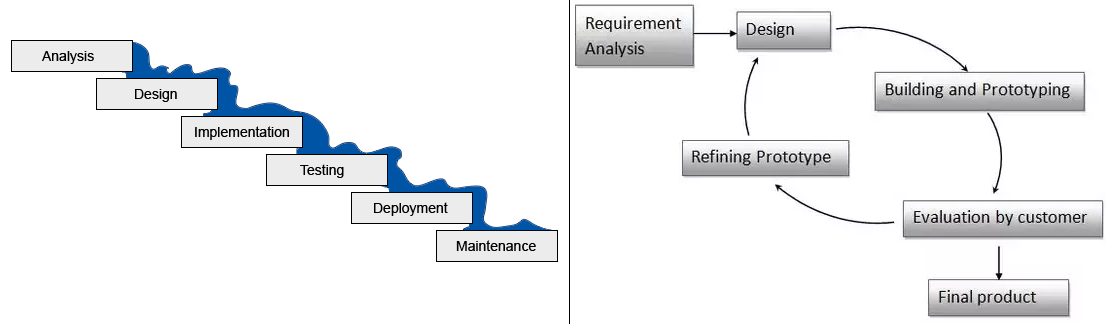
\includegraphics[width=.6\textwidth]{resources/warterfall_prototype}\\
	\caption{The Waterfall and Prototype SDLC models}
\end{figure}

%https://www.iso.org/obp/ui/#iso:std:iso-iec:tr:24774:ed-2:v1:en
%https://www.iso.org/standard/53815.html
Every company may use it's own SDLC model, there is a standard that presents guidelines for the elements used most frequently in describing a process: the title, purpose, outcomes, activities, task and information item

The complexity and slowness in producing a concrete product in other SDLC brought the need for a faster and more communicative model.
%https://www.tutorialspoint.com/sdlc/sdlc_agile_model.htm
Agile SDLC model is a combination of iterative and incremental process models with focus on process adaptability and customer satisfaction by rapidly and continuously deliver of working software product.

This chapter describes the most fundamental points of the Agile method, how it started and the adaptations that derived from it, like Scrum.
At the end, it also explains how Athonet's adaptation of the Agile life cycle works.

\section{Why the need for another software lifecycle}
%https://techbeacon.com/app-dev-testing/agility-beyond-history-legacy-agile-developmentdl

	The decade of 1990 represented a very important turning point for the computer industry.
	Computers were spreading everywhere and the software companies faced the so called application development crisis.
	
	The problem was that businesses moved too fast and within the space of three years, requirements, systems, and even entire businesses were likely to change.
	%todo change
	That meant that many projects ended up being cancelled partway through, and many of those that were completed didn't meet all the business's current needs, even if the project's original objectives were met.

	The Space Shuttle program, which operationally launched in 1982, used information and processing technologies from the 1960s.
	
%	https://hackr.io/blog/sdlc-methodologies
	SDLC models can be of two types:
	\begin{itemize}
		\item Iterative: (like ..)
		\item Incremental: (like .. )
	\end{itemize}
	
	The most used models before Agile were Waterfall and X
	
	The pros / cons of waterfall were ... 
	The pros / cons of x where ...

	The excessive documentation and little communication with the client brought to the need of a new model that prioritizes the product and the people over bureaucracy. 

	Jon Kern, an aerospace engineer in the 1990s, became increasingly frustrated with these long lead times and with the decisions made early in a project that couldn't be changed later. "We were looking for something that was more timely and responsive," he notes, joining a growing number of those who felt that there had to be a better way to build software. He was one of 17 software thought leaders who started meeting informally and talking about ways to develop software more simply, without the process and documentation overhead of waterfall and other popular software engineering techniques of the time.
	These frustrations around seemingly unproductive software development activities, which were shared by like-minded professionals, led to the now-famous Snowbird meeting in Utah in early 2001.
	Perhaps various agile and iterative techniques would still be in the minority were it not for the Agile Manifesto, codified at that 2001 meeting in Snowbird.

% https://agilemanifesto.org/
%https://www.productplan.com/glossary/agile-manifesto/
\section{The Agile manifesto}

	The Agile Manifesto is a brief document built on 4 values and 12 principles for agile software development. The Agile Manifesto was published in February 2001 and is the work of 17 software development practitioners who observed the increasing need for an alternative to documentation-driven and heavyweight software development processes.
	
	The 4 values are:
	\begin{itemize}
		\item Individuals and interactions over processes and tools
		\item Working software over comprehensive documentation
		\item Customer collaboration over contract negotiation
		\item Responding to change over following a plan
	\end{itemize}

	These 12 principles emphasize things like “early and continuous delivery of valuable software” and “continuous attention to technical excellence”.
	
	The 12 principles are:
	Our highest priority is to satisfy the customer
	through early and continuous delivery
	of valuable software.
	
	Welcome changing requirements, even late in
	development. Agile processes harness change for
	the customer's competitive advantage.
	
	Deliver working software frequently, from a
	couple of weeks to a couple of months, with a
	preference to the shorter timescale.
	
	Business people and developers must work
	together daily throughout the project.
	
	Build projects around motivated individuals.
	Give them the environment and support they need,
	and trust them to get the job done.
	
	The most efficient and effective method of
	conveying information to and within a development
	team is face-to-face conversation.
	
	Working software is the primary measure of progress.
	
	Agile processes promote sustainable development.
	The sponsors, developers, and users should be able
	to maintain a constant pace indefinitely.
	
	Continuous attention to technical excellence
	and good design enhances agility.
	
	Simplicity--the art of maximizing the amount
	of work not done--is essential.
	
	The best architectures, requirements, and designs
	emerge from self-organizing teams.
	
	At regular intervals, the team reflects on how
	to become more effective, then tunes and adjusts
	its behavior accordingly.
	
	* 
	
	All of them are important but, in my opinion, the ones that most important ones are ... because they represent the intent of placing the product and the customer above everything else.

% Agile adaptations
\section{Agile's little big cousins}
	
	While the 12 agile principles and 4 values for agile provide useful guidance for those hoping to practice agile software development, they are not prescriptive.
	The Agile Manifesto does not outline any specific processes, procedures, or best practices for agile. And that is intentional. The creators did not set out to develop a rigid framework or methodology. Instead, they created a philosophical mindset for software development.

	%https://scrumstar.com/articles/the-most-popular-agile-methodologies
	This allowed the creation of derivates like:
	\begin{itemize}
		\item ...
	\end{itemize}\\
	kanban, scrum, etc.

%	https://explore.versionone.com/state-of-agile

Reasons for Adopting Agile
The reasons stated for adopting agile were less about increasing
productivity (51% compared to 55% last year), and more about
improving team morale (34% compared to 28% last year) and
less about reducing project risk (28% compared to 37% last
year), and more about reducing project costs (41% compared to
24\% last year).

95\% of respondents reported at least some of their agile projects have been successful with 48% reporting that most or all of
their agile projects were successful.

Business value delivered
and Customer/user
satisfaction remained the
top two cited measures
of success for individual
projects in this year’s
survey. Earned value went
from 8\% last year to 12\%
this year.

Jira 65\%

	According to a survey from mid 2018 that analyzes the market share of the most used Agile derivatives, 'Agile is a blanket term that describes a set of software development principles'.
	



	
% SPOTIFY
%https://medium.com/@media_75624/exploring-key-elements-of-spotifys-agile-scaling-model-471d2a23d7ea
%https://medium.com/productmanagement101/spotify-squad-framework-part-i-8f74bcfcd761

% AMAZON
%https://www.forbes.com/sites/stevedenning/2019/06/02/how-amazon-became-agile/

% MICROSOFT
%https://www.forbes.com/sites/stevedenning/2015/10/27/surprise-microsoft-is-agile/

% NETFLIX
%https://smartbear.com/blog/develop/5-lessons-agile-teams-can-learn-from-netflix/
%http://www.agileadvice.com/2018/03/02/profiles/a-case-study-of-netflixs-high-performance-culture/

LSD (Lean Software Development)
This methodology is an adaptation of the Toyota lean manufacturing principles to software development. It was introduced in 2009 by Marry and Tom Poppendieck in their book "Lean Software Development: An Agile Toolkit."

\section{Agile in small companies}
	e le piccole aziende come athonet come fanno? (misto)

\section{The advantages and disadvantafes of Agile}
	l'agile può andare a completamente sostituire il resto\\
	cosa ne pensano gli utenti

\section{What Agile variant will Athonet use}
	misto a causa dei pochi dipendenti che hanno ancora una responsabilità ampia all'interno dell'azienda ma pensano che si possa incorporare agile\\
	processi di business

